\documentclass[a4paper,11pt]{article}\usepackage[]{graphicx}\usepackage[]{color}
%% maxwidth is the original width if it is less than linewidth
%% otherwise use linewidth (to make sure the graphics do not exceed the margin)
\makeatletter
\def\maxwidth{ %
  \ifdim\Gin@nat@width>\linewidth
    \linewidth
  \else
    \Gin@nat@width
  \fi
}
\makeatother

\definecolor{fgcolor}{rgb}{0.345, 0.345, 0.345}
\newcommand{\hlnum}[1]{\textcolor[rgb]{0.686,0.059,0.569}{#1}}%
\newcommand{\hlstr}[1]{\textcolor[rgb]{0.192,0.494,0.8}{#1}}%
\newcommand{\hlcom}[1]{\textcolor[rgb]{0.678,0.584,0.686}{\textit{#1}}}%
\newcommand{\hlopt}[1]{\textcolor[rgb]{0,0,0}{#1}}%
\newcommand{\hlstd}[1]{\textcolor[rgb]{0.345,0.345,0.345}{#1}}%
\newcommand{\hlkwa}[1]{\textcolor[rgb]{0.161,0.373,0.58}{\textbf{#1}}}%
\newcommand{\hlkwb}[1]{\textcolor[rgb]{0.69,0.353,0.396}{#1}}%
\newcommand{\hlkwc}[1]{\textcolor[rgb]{0.333,0.667,0.333}{#1}}%
\newcommand{\hlkwd}[1]{\textcolor[rgb]{0.737,0.353,0.396}{\textbf{#1}}}%

\usepackage{framed}
\makeatletter
\newenvironment{kframe}{%
 \def\at@end@of@kframe{}%
 \ifinner\ifhmode%
  \def\at@end@of@kframe{\end{minipage}}%
  \begin{minipage}{\columnwidth}%
 \fi\fi%
 \def\FrameCommand##1{\hskip\@totalleftmargin \hskip-\fboxsep
 \colorbox{shadecolor}{##1}\hskip-\fboxsep
     % There is no \\@totalrightmargin, so:
     \hskip-\linewidth \hskip-\@totalleftmargin \hskip\columnwidth}%
 \MakeFramed {\advance\hsize-\width
   \@totalleftmargin\z@ \linewidth\hsize
   \@setminipage}}%
 {\par\unskip\endMakeFramed%
 \at@end@of@kframe}
\makeatother

\definecolor{shadecolor}{rgb}{.97, .97, .97}
\definecolor{messagecolor}{rgb}{0, 0, 0}
\definecolor{warningcolor}{rgb}{1, 0, 1}
\definecolor{errorcolor}{rgb}{1, 0, 0}
\newenvironment{knitrout}{}{} % an empty environment to be redefined in TeX

\usepackage{alltt}

\usepackage{amsmath,amssymb,amsfonts,amsthm}    % Typical maths resource packages
\usepackage{graphicx}                           % Packages to allow inclusion of graphics
\usepackage{hyperref}                           % For creating hyperlinks in cross references
\usepackage[ngerman]{babel}
\usepackage[backend=bibtex, style=authoryear, language=ngerman, isbn=false, url=false, doi=false, eprint=false, natbib=true, citestyle=authoryear]{biblatex}
\usepackage[utf8]{inputenc}
\usepackage{hyperref}

\bibliography{Bibliographie}
% -------------------------------
% --- some layout definitions ---
% -------------------------------

% define topline
\usepackage[automark]{scrpage2}
\pagestyle{scrheadings}
\automark{section}
\clearscrheadings
\ohead{\headmark}

% define page size, margin size
\setlength{\headheight}{2\baselineskip}
\voffset=-2cm
\hoffset=-3cm
\textheight24cm
\textwidth15.5cm
\topmargin1cm
\oddsidemargin3cm
\evensidemargin3cm

\renewcommand{\baselinestretch}{1.5}
\renewcommand{\labelitemii}{-}
\IfFileExists{upquote.sty}{\usepackage{upquote}}{}
\begin{document}










% -------------------------------
% --- frontmatter: Title page ---
% -------------------------------

\thispagestyle{empty}
\begin{center}
    {\normalsize{\bf Masterarbeit}} \\\vspace{0.5cm}
    {\Large{\bf Aufwertung und Verdrängung in Berlin: \\
                Räumliche Analysen zur Messung von Gentrifizierung}} \vspace{1.0cm}

    {\normalsize eingereicht beim Betreuer}\\\vspace{0.5cm}
    {\normalsize{\bf Prof. Dr. Axel Werwatz}} \\\vspace{0.5cm}
    {\normalsize Technische Universität Berlin \\
    Fakultät VII - Wirtschaft und Management \\
    Institut für Volkswirtschaftslehre und Wirtschaftsrecht \\
    FG Ökonometrie und Wirtschaftsstatistik} \vspace{1cm}

    {\normalsize sowie beim Zweitgutachter}\\\vspace{0.5cm}
    {\normalsize{\bf Dr. Andrej Holm}} \\\vspace{0.5cm}
    {\normalsize Humboldt-Universität zu Berlin \\
    Kultur-, Sozial- und Bildungswissenschaftliche Fakultät\\
    Institut für Sozialwissenschaften\\
    Stadt- und Regionalsoziologie} \vspace{1cm}

    {\normalsize vorgelegt von \\\vspace{0.5cm}
    {\bf Guido Schulz} \\
    Matrikelnummer: HU 554142 \\
    \href{mailto:schulzgu@student.hu-berlin.de}{schulzgu@student.hu-berlin.de}} \vspace{1cm}


    {\normalsize Zur Erlangung des akademischen Grades eines \\
    {\bf Master of Science (M.Sc.) in Statistik} \\
    Berlin, den 25. August 2015}

\end{center}


% ------------------------------------
% --- frontmatter: Acknowledgement ---
% ------------------------------------
\newpage
\pagestyle{plain}
\pagenumbering{roman}   % define page number in roman style
\setcounter{page}{1}    % start page numbering
\section*{Danksagung}

I would like to thank




% -----------------------------
% --- frontmatter: Abstract ---
% -----------------------------
\newpage

\selectlanguage{ngerman} 
\begin{center}
     {\Large{\bf Aufwertung und Verdrängung in Berlin: \\
                Räumliche Analysen zur Messung von Gentrifizierung}} \vspace{1.0cm} \\
    {\bf Guido Schulz} \\ \vspace{2cm}

\begin{abstract}
Trotz des "`boomenden"' Berliner Immobilienmarktes, der großen medialen Aufmerksamkeit für das Thema der Gentrifizierung und den von stadtpolitischen Protestbewegungen kritisierten sozialen Auswirkungen von Aufwertungsprozessen, wurden in Berlin bisher kaum Studien zur Messung von Gentrifizierung unternommen. Mit dem Versuch einer stadtweit kleinräumigen Erfassung von Aufwertung und Verdrängung soll mit dieser Arbeit sowohl zur Schließung der Lücke in der deutschen Literatur zu Gentrifizierung, als auch zur Behebung methodischer Mängel vergleichbarer internationaler Studien beigetragen werden. Durch die Analyse von Aggregatsdaten des Beobachtungszeitraums von 2007-2012 konnten mithilfe eigens (weiter)entwickelter deskriptiver wie inferentieller statistischer Methoden Gentrifizierungsgebiete auf Nachbarschaftsniveau identifiziert und vergleichend charakterisiert werden. Überdies konnte ein starker Zusammenhang zwischen Aufwertung und Verdrängung nachgewiesen werden. So konnte gezeigt werden, dass die Gentrifizierungsgebiete im Vergleich zu entsprechenden Kontrollgebieten viel höhere Binnenfortzugs- und Außenzuzugsraten besaßen. Im Zusammenhang mit den dort vorherrschenden, intensiven sozialen und immobilienwirtschaftlichen Aufwertungsdynamiken ließ dies auf eine Verdrängung ärmerer Bevölkerungsgruppen schließen. Zudem ergab eine über gewichtete, räumlich autoregressive Modelle (SAR) ermittelte Schätzung ökonomischer Verdrängungsraten ähnliche Werte, wie sie von Newman und Wyly im Jahre 2006 für New York City errechnet wurden.
\end{abstract}

\newpage
\selectlanguage{english} 
{\Large{\bf Valorisation and Displacement in Berlin: \\
                Spatial Analyses for Measuring Gentrification}} \vspace{1.0cm} \\
     {\bf Guido Schulz} \\ \vspace{2cm}

\begin{abstract}
The real-estate market in Berlin is booming, the issue of gentrification has recently received increased media interest and urban protest movements are condemning the social consequences of real-estate valorisation. Despite all this attention, research on measuring gentrification in Berlin has been scarce. By attempting to capture real-estate valorisation and its associated social upgrading and displacement processes, this study sought to close a gap in the German gentrification literature and also aimed to resolve methodological shortcomings of comparable international studies. By refining and developing descriptive as well as inferential statistical methods applied to aggregate data from 2007-2012, neighbourhoods experiencing gentrification could be identified and characterized. Furthermore, a strong relationship between real-estate valorisation and displacement could be verified. A comparison between gentrification and control areas revealed that the gentrification areas exhibit much higher mobility rates. Given the intense dynamics of social upgrading and real-estate valorisation in these areas, the high mobility rates strongly suggested that financially disadvantaged residents were being displaced. In addition, an estimation of economic displacement rates via weighted Spatially Autoregressive Models (SAR) yielded similar values to those Newman and Wyly had calculated for New York City back in 2006.
\end{abstract}
\end{center} 
\selectlanguage{ngerman}


% -----------------------------
% --- frontmatter: Contents ---
% -----------------------------
\newpage
\tableofcontents
\clearpage



% ----------------------------------------------------
% --- frontmatter: List of Figures (not mandatory) ---
% ----------------------------------------------------
\newpage
\addcontentsline{toc}{section}{Abkürzungsverzeichnis}
\ohead[]{Abkürzungsverzeichnis}
\section*{Abkürzungsverzeichnis}

\begin{tabular}{rp{0.2cm}lp{1cm}rp{0.2cm}l}
    CPI     & &  Consumer Price Index   & & ETF     & &  Equity Traded Funds  \\
    ETH     & &  Eat the Horse          & & XLM     & &  Xetra Liquidity
\end{tabular}




% ----------------------------------------------------
% --- frontmatter: List of Figures (not mandatory) ---
% ----------------------------------------------------
\newpage
\addcontentsline{toc}{section}{Abbildungsverzeichnis}
\ohead[]{\rightmark}
\listoffigures



% ---------------------------------------------------
% --- frontmatter: List of Tables (not mandatory) ---
% ---------------------------------------------------
\newpage
\addcontentsline{toc}{section}{Tabellenverzeichnis}
\listoftables



% -------------------------------
% --- main body of the thesis ---
% -------------------------------
\newpage
\pagestyle{plain}
\setcounter{page}{1}    % start page numbering anew
\pagenumbering{arabic}  % page numbers in arabic style


\section{Einleitung}
 Berliner Wohnungsmarkt

"`Der Berliner Wohnungsmarkt ist in den letzten Jahren durch fast flächendeckende Mietsteigerungen geprägt und innerhalb des S-Bahn-Rings hat sich Gentrification zu einem Mainstream-Phänomen entwickelt."' \citep[S.~29]{Berner2015}
"`Capital accumulation through real-estate activity booms"' schrieb \citet[S.~35]{Harvey2008} über Mumbai. Über Berlin hätte er das wohl im Jahre 2008 noch nicht geschrieben, denn der Boom des Immoblienmarktes ist in Berlin erst mit etwas Verzögerung ist Berlin angekommen. im Integration in globale zweite Zirkulationsphäre Finanzkapitals. Krisenanlagen, Spatial fix "`Betongold"' Europäische Krise 

Investitionen nicht notwendig für Aufwertung, da 
Hiermit ist nicht notwendigerweise eine bauliche Aufwertung gemeint. In Berlin auf immobilienwirtschaftliche Aufwertung auch ohne bauliche Aufwertung möglich \citep[S.~30]{Berner2015} 

 

\begin{itemize}

\item \textit{Gestiegene Nachfrage} \\
  Berlin besitzt seit 2001 jedes Jahr ein positives Wanderungssaldo mit stark steigendem Trend \citep{StatistischesLandesamtSachsen-Anhalt2015}. Einen extremer Anstieg des Wanderungssaldos ist für den Zeitraum von 2009 bis 2011 zu beobachten. In nur 2 Jahren kam es zu einer Zunahme des Wanderungssaldos von 3,1 je 1000 Einwohner auf 12 je 1000 Einwohner an - es vervierfachte sich also fast. Während Anfang der 2000er Jahre noch ein ein mittlerweile niedrige Leerstandsquoten (Verweis), Umwandlungen in Eigentumswohnungen im Bestand verringert das verschärft die Angebotslücke an Mietwohnungen
  \item \textit{Niedrige Neubautätigkeit}\\
    Obwohl in bestimmten Nachbarschaften Berlins Aufwertungsprozesse auch entscheidend durch Neubautätigkeiten getragen werden können (\textit{Neubau-Gentrification}), so ist bei der vorherrschend niedrigen Neubauquote und dem relativ niedrigem Invesitionsvolumen nicht davon auszugehen, Bestandsquartiere wie Prenzlauerberg, Friedrichshain oder Kreuzberg.  dass die davon auszugehen, dass Hier Zahlen von niedriger Neubauquote und niedrigem Investitionsvolumen 
   Neubau ist Eigentumswohnungen und ein "`hoher Anteil der gerade fertiggestellten Neubauwohnungen befindet sich im Top-Segment"' (Wohnungsmarktbericht 2014) Im Jahre 2013 
   Etwa 14 Prozent der Objekte sind als Mietwohnungsbauten konzipiert oder weisen sowohl Eigentums- als auch Mietwohnungen auf



    \item What is the subject of the study? Describe the
        economic/econometric problem.
    \item What is the purpose of the study (working hypothesis)?
    \item What do we already know about the subject (literature
        review)? Use citations: shows that...
        Alternative Forms of the Wald test are considered
    \item What is the innovation of the study?
    \item Provide an overview of your results.
    
"`I would challenge [...] anyone to show how census data can provide convincing evidence of displacement. It can show that one class or housing tenure has grown and that another has declined but it cannot show displacement."' Hamnet 2010 S.~184

Gentrimap beinhaltet keine Analyse von zwischen Aufwertungsprozessen und Wanderungsverhalten.

Versuch Verdrängung in Berlin im Zweitraum zwischen 2007-2012 statistisch kleinräumlig zu erfassen und 


"`it is essential to have conceptual clarity before research on displacement begins, and before any conclusions can be drawn"' \citet[S.~304]{Slater2009}

Eine Analyse (von altgriech analysis „Auflösung“) ist eine systematische Untersuchung, bei der das untersuchte Objekt oder Subjekt in Bestandteile (Elemente) zerlegt und auf Grundlage von Kriterien erfasst werden. Anschließend werden diese geordnet, untersucht und ausgewertet. Insbesondere betrachtet man Beziehungen und Wirkungen (oft: Wechselwirkungen) zwischen den Elementen.

"`Eine Analyse (von altgriech analysis 'Auflösung') ist eine systematische Untersuchung, bei der das untersuchte Objekt oder Subjekt in Bestandteile (Elemente) zerlegt und auf Grundlage von Kriterien erfasst werden. Anschließend werden diese geordnet, untersucht und ausgewertet. Insbesondere betrachtet man Beziehungen und Wirkungen (oft: Wechselwirkungen) zwischen den Elementen."' Wikipedia



Verdrängung messen:
Probleme: Slater 2009 "`there is no such data"' und gleichzeitig sagt er Slater 2015 über die Schwierigkeiten Gentrificationtheorie zu operationalisieren "`theories are always confronted with empirical difficulties. They should not be abandoned because of it."'


Keine qualitativen Methoden, 

Stadteweite, kleinräumige Zensusdaten Aufwertung wohnräumliche Mobilität
Deskriptiv Explorative Datenanalyse: Charakterisierung  
Inferenziell Räumlich Autoregressive Modelle

Durch die statistische Modellierung des Zusammenhang zwischen immoblienwirtschaftlichen sowie sozialen Aufwertungsprozessen und wohnräumlicher Mobilität sollen empirische Erkenntnisse bezüglich der Existenz, Lokalisierung und Quantifizierung von Gentrification und Verdrängung in Berlin gewonnen werden. \\
Zunächst soll mit Hilfe stadtsoziologischer Theorie der konzeptionelle Rahmen für die Studie bestimmt und Begriffsdefinitionen gesetzt werden. Auf Grundlage des aktuellen Forschungsstandes werden Forschungsfragen entwickelt und Hypothesen formuliert. \\
Im ersten Schritt sollen mit den Methoden explorativer Datenanalyse eine räumliche Identifizierung und Quantifizierung von Gentrificationprozessen in Berlin vorgenommen werden. Die identifizierten Aufwertungsgebiete werden in einem Vergleich mit entsprechenden Kontrollgebieten genauer charaktierisiert. In einem zweiten Schritt werden räumlich autoregressive Modelle \textit{(\ac{SAR})} geschätzt um einerseits den Effekt immobilienwirtschaftlicher Aufwertungsdynamik auf die wohnräumliche Mobilität der Berliner Bevölkerung zu messen und andereseits um den Charakter und Ausmaß der Interaktion zwischen sozialer Aufwertungsdynamik und wohnräumlicher Mobilität zu bestimmen. Die Ergebnisse der Regressionsmodelle werden dann im Kontext Marcuses Verdrängungstypen intepretiert und analysiert.
\end{itemize}






\section{Method/Model/Theory}\label{Sec:Method}

\begin{itemize}

    \item How was the data analyzed ?

    \item Present the underlying economic model/theory and
        give reasons why it is suitable to answer the given problem.

    \item Present econometric/statistical estimation method and
        give reasons why it is suitable to answer the given problem.

    \item Allows the reader to judge the validity of the study and
        its findings.

    \item Depending on the topic this section can also be split up
        into separate sections.

\begin{knitrout}
\definecolor{shadecolor}{rgb}{0.969, 0.969, 0.969}\color{fgcolor}
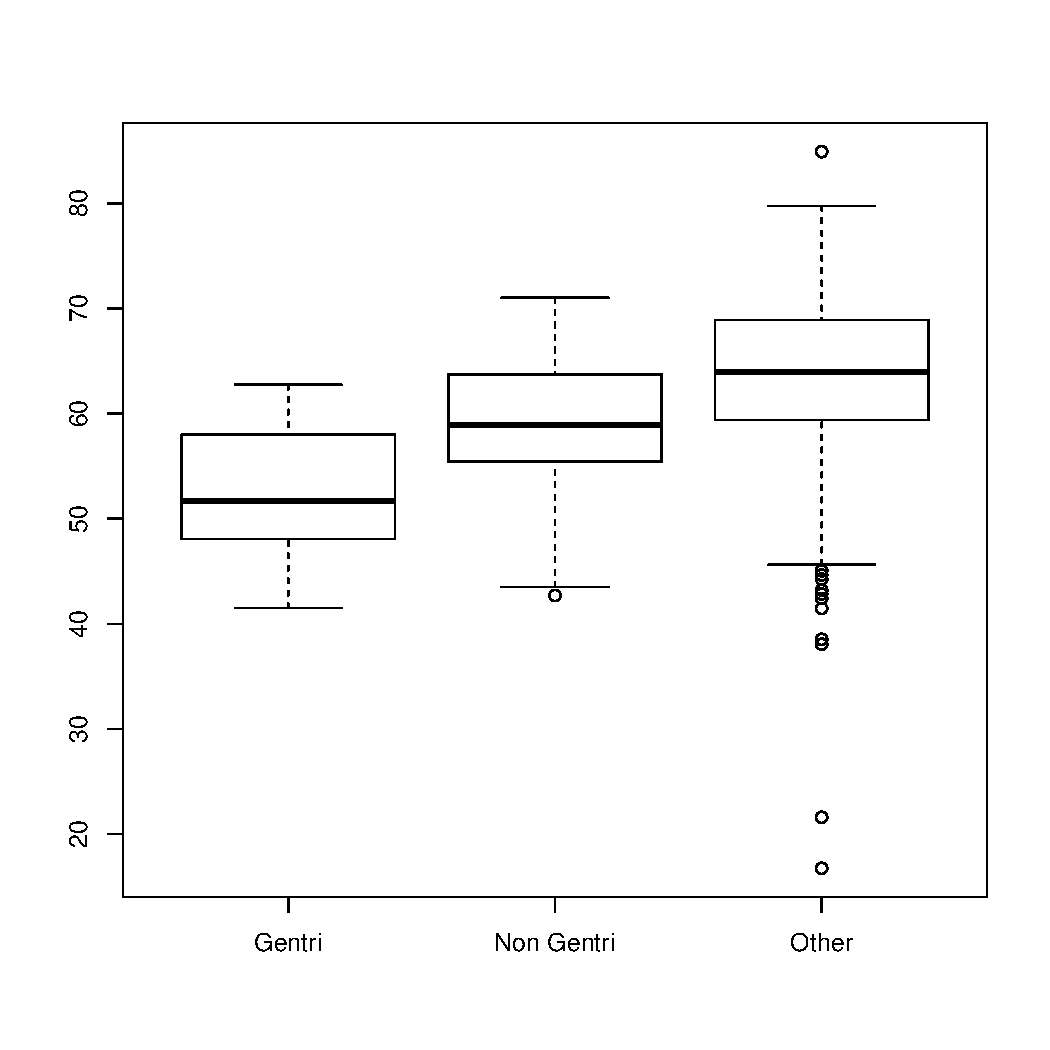
\includegraphics[width=\maxwidth]{figure/unnamed-chunk-3-1} 

\end{knitrout}


\end{itemize}

\newpage





\section{Data}\label{Sec:Data}

\begin{itemize}

    \item Describe the data and its quality.
    \item How was the data sample selected?
    \item Provide descriptive statistics such as:
        \begin{itemize}
            \item time period,
            \item number of observations, data frequency,
            \item mean, median,
            \item min, max, standard deviation,
            \item skewness, kurtosis, Jarque--Bera statistic,
            \item time series plots, histogram.
        \end{itemize}
    \item For example:
        \begin{table}[ht]
        \begin{center}
            {\footnotesize
            \begin{tabular}{l|cccccccccc}
                \hline \hline
                           & 3m    & 6m    & 1yr   & 2yr   & 3yr   & 5yr   & 7yr   & 10yr  & 12yr  & 15yr   \\
                \hline
                    Mean   & 3.138 & 3.191 & 3.307 & 3.544 & 3.756 & 4.093 & 4.354 & 4.621 & 4.741 & 4.878  \\
                    StD    & 0.915 & 0.919 & 0.935 & 0.910 & 0.876 & 0.825 & 0.803 & 0.776 & 0.768 & 0.762  \\
                \hline \hline
            \end{tabular}}
        \end{center}
        \caption{Some descriptive statistics of location and dispersion for
        2100 observed swap rates for the period from February 15, 1999
        to March 2, 2007. Swap rates measured as 3.12 (instead of 0.0312). See Table
        \ref{Tab:DescripStatsRawDataDetail} in the appendix for
        more details.}
        \label{Tab:DescripStatsRawData}
        \end{table}

    \item Allows the reader to judge whether the sample is biased or to evaluate possible impacts of outliers, for
    example.
    
\begin{knitrout}
\definecolor{shadecolor}{rgb}{0.969, 0.969, 0.969}\color{fgcolor}\begin{kframe}
\begin{verbatim}
##       PLZ            Zeit         Miete_H1         Miete_H2     
##  10115  :  11   Min.   :2004   Min.   : 3.700   Min.   : 3.800  
##  10117  :  11   1st Qu.:2006   1st Qu.: 5.500   1st Qu.: 5.500  
##  10119  :  11   Median :2009   Median : 6.300   Median : 6.400  
##  10178  :  11   Mean   :2009   Mean   : 6.586   Mean   : 6.712  
##  10179  :  11   3rd Qu.:2012   3rd Qu.: 7.300   3rd Qu.: 7.500  
##  10243  :  11   Max.   :2014   Max.   :14.000   Max.   :14.000  
##  (Other):2024                  NA's   :34       NA's   :27
\end{verbatim}
\end{kframe}
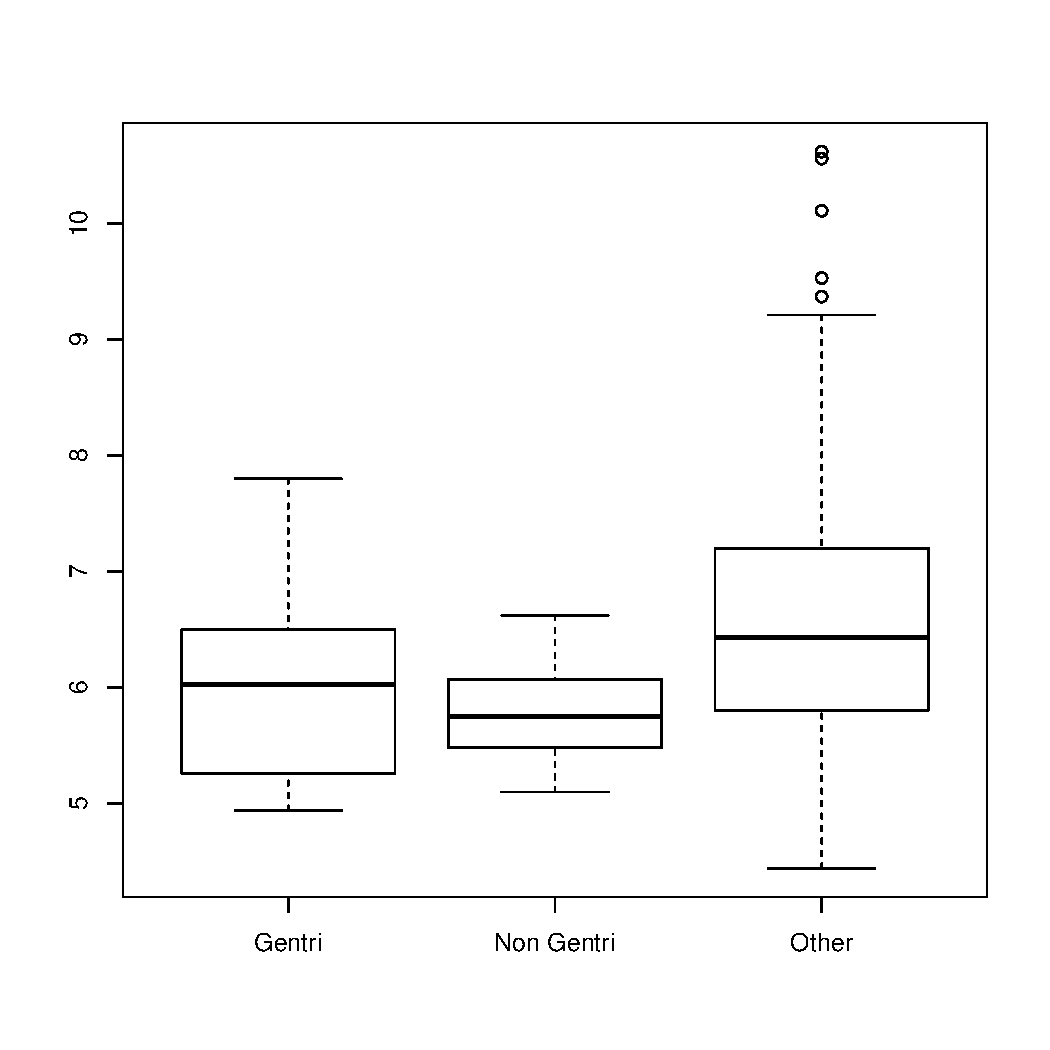
\includegraphics[width=\maxwidth]{figure/unnamed-chunk-4-1} 

\end{knitrout}

\cite{Wyly2010} is auchs schön

\end{itemize}

\newpage





\section{Results}\label{Sec:Results}

\begin{itemize}

    \item Organize material and present results.

    \item Use tables, figures (but prefer visual presentation):
        \begin{itemize}
            \item Tables and figures should supplement (and not duplicate) the
                text.

            \item Tables and figures should be provided with
            legends.\\

            \item Tables and graphics may appear in the text or in
                the appendix, especially if there are many simulation results
                tabulated, but is also depends on the study and number of tables resp.
                figures. The key graphs and tables must appear in
                the text!
        \end{itemize}

    \item Latex is really good at rendering formulas:\\
        {\it Equation (\ref{Eq:SpecDens}) represents the ACs of a stationary
        stochastic process:
        \begin{equation}
            f_y(\lambda) = (2\pi)^{-1} \sum_{j=-\infty}^{\infty}
                           \gamma_j e^{-i\lambda j}
                         =(2\pi)^{-1}\left(\gamma_0 + 2 \sum_{j=1}^{\infty}
        \gamma_j \cos(\lambda j)\right)
                                        \label{Eq:SpecDens}
        \end{equation}
        where $i=\sqrt{-1}$ is the imaginary unit, $\lambda \in [-\pi,
        \pi]$ is the frequency and the $\gamma_j$ are the autocovariances
        of $y_t$.}

\newpage

    \item Discuss results:
        \begin{itemize}
            \item Do the results support or do they contradict economic theory ?
            \item What does the reader learn from the results?
            \item Try to give an intuition for your results.
            \item Provide robustness checks.
            \item Compare to previous research.
        \end{itemize}
\end{itemize}


This document was produced in RStudio using the knitr package \citep{Robson2009}.
\nocite{Freeman2005}
\citet{Freeman2005} is auch schön
 


% ----------------
% --- appendix ---
% ----------------
\appendix

% literature
\newpage
\addcontentsline{toc}{section}{Literatur}

\printbibliography


% figures (not mandatory)
\newpage
\section{Abbildungen}

hier kommen dann die Abbildungen hin


% tables (not mandatory)
\newpage
\newpage
\section{Tabellen}

\begin{table}[h]
\centering
\begin{tabular}{@{}lrrrr@{}}
\toprule
                                       & \multicolumn{1}{r}{{\bf Gentri}} & \multicolumn{1}{r}{{\bf Kontroll}} & \multicolumn{1}{r}{{\bf Andere}} & \multicolumn{1}{r}{{\bf \textit{Gesamt}}} \\ \midrule
$m$                                    & 45                               & 139                                & 246                              & 430                                  \\
$Q_{0.5}(EW_{2007})$                   & 9734                             & 7172                               & 6309                             & 6907                                 \\
$\Sigma\;EW_{2007}$                    & 456355                           & 1158061                            & 1727819                          & 3342235                              \\ \bottomrule
\end{tabular}
\caption{Statistiken zur Einwohner*innenzahl 2007 nach \textit{Kategorie}}\label{tab:KategorieEW}
\end{table}            

\begin{table}[h]
\centering
\begin{tabular}{@{}lrrrrrr@{}}
\toprule
               & $min$ & $Q_{0,25}$ & $Q_{0,5}$ & $Q_{0,75}$ & $max$ & $mean$ \\ \midrule
{\bf Gentri}   & 5,38 & 11,32 & 12,47 & 13,37 & 15,77 & 12,39 \\
{\bf Kontroll} & 5,73 &  8,33 &  9,53 & 10,68 & 14,40 & 9,62 \\ \bottomrule
\end{tabular}
\caption{Deskriptive Statistiken von \textit{Fortzüge} für Gentrification- und Kontrollgebiete}
\label{tab:FortzuegeR}
\end{table}

\begin{table}[h]
\centering
\begin{tabular}{@{}lrrrrrr@{}}
\toprule
               & $min$ & $Q_{0,25}$ & $Q_{0,5}$ & $Q_{0,75}$ & $max$ & $mean$ \\ \midrule
{\bf Gentri}   & 7,98 & 10,10 & 10,88 & 12,27 & 21,07 & 11,00 \\
{\bf Kontroll} & 6,93 & 8,77 & 9,47 & 10,75 & 14,43 &  9,80  \\ \bottomrule
\end{tabular}
\caption{Deskriptive Statistiken von \textit{Zuzüge} für Gentrification- und Kontrollgebiete}
\label{tab:ZuzuegeR}
\end{table}

\begin{table}[h]
\centering
\begin{tabular}{@{}lrrrrrr@{}}
\toprule
               & $min$ & $Q_{0,25}$ & $Q_{0,5}$ & $Q_{0,75}$ & $max$ & $mean$ \\ \midrule
{\bf Gentri}   & 1,97 & 4,53 & 5,22 & 5,93 & 6,83  & 5,18 \\
{\bf Kontroll} & 1,42 & 2,53 & 3,22 & 4,32 & 8,85  & 3,51 \\ \bottomrule
\end{tabular}
\caption{Deskriptive Statistiken von \textit{FortzügeA} für Gentrification- und Kontrollgebiete}
\label{tab:FortzuegeUDAR}
\end{table}

\begin{table}[h]
\centering
\begin{tabular}{@{}lrrrrrr@{}}
\toprule
               & $min$ & $Q_{0,25}$ & $Q_{0,5}$ & $Q_{0,75}$ & $max$ & $mean$ \\ \midrule
{\bf Gentri}   & 2,77  & 5,62       & 6,92      & 7,83       & 12,52 & 6,90   \\
{\bf Kontroll} & 1,20  & 2,63       & 3,65      & 5,32       & 11,37 & 4,09   \\ \bottomrule
\end{tabular}
\caption{Deskriptive Statistiken von \textit{ZuzügeA} für Gentrification- und Kontrollgebiete}
\label{tab:ZuzuegeUDAR}
\end{table}






% --------------------------------------------
% --- last page: Declaration of Authorship ---
% --------------------------------------------

\newpage
\thispagestyle{empty}
%{\Large{\bf Declaration of Authorship}}\vspace{0.5cm}

\section*{Eigenständigkeitserklärung}

Ich erkläre ausdrücklich, dass es sich bei dieser Abschlussarbeit um eine von mir erstmalig, selbstständig und ohne fremde Hilfe verfasste Arbeit handelt. Ich erkläre ausdrücklich, dass ich sämtliche in der oben genannten Arbeit
verwendeten fremden Quellen, auch aus dem Internet (einschließlich Tabellen,
Grafiken u. Ä.) als solche kenntlich gemacht habe. Insbesondere bestätige ich,
dass ich ausnahmslos sowohl bei wörtlich übernommenen Aussagen bzw.
unverändert übernommenen Tabellen, Grafiken u. Ä. (Zitaten) als auch bei in
eigenen Worten wiedergegebenen Aussagen bzw. von mir abgewandelten
Tabellen, Grafiken u. Ä. anderer Autorinnen und Autoren (Paraphrasen) die
Quelle angegeben habe. Mir ist bewusst, dass Verstöße gegen die Grundsätze der Selbstständigkeit als
Täuschung betrachtet und entsprechend der fachspezifischen Prüfungsordnung
und/oder der Allgemeinen Satzung für Studien- und Prüfungsangelegenheiten
der HU (ASSP) bzw. der Fächerübergreifenden Satzung zur Regelung von
Zulassung, Studium und Prüfung der Humboldt-Universität (ZSP-HU) geahndet
werden.

\vspace{1cm}

Berlin, den 25. August 2015 \vspace{1.5cm}

Guido Schulz


\end{document}
